\section{Les hypercubes}

Un hypercube est une grille de dimension $d$ ne possédant que deux sommets selon chaque coordonnée. Ainsi, il possède $2^d$ nœuds de degré $d$ et $d2^{d-1}$ arêtes. On construit un hypercube de dimension $d$ récursivement à partir de deux hypercubes de dimension $d-1$ en connectant les sommets similaires, un hypercube de dimension 0 correspondant à un nœud de calcul unique. On obtient ainsi ces quatre premières grilles :
\\
\begin{figure}[!h]
\begin{center}
\hspace*{-1.2in}
\begin{tabular}{ccccccccc}
~~	$d = 0$ & & ~~ $d = 1$ & & ~~~$d = 2$ & & $d = 3$ & & ~~~~~~~~~~~~~~~~~~~~~~~~~~~~~~~~$d = 4$ \\ 
\begin{minipage}[c]{0.02\linewidth}
\begin{center}
\begin{tikzpicture}
\SetGraphUnit{1}
\GraphInit[vstyle=Normal]
\SetUpVertex[FillColor=blue!20]
\Vertex{}
\end{tikzpicture}
\end{center}
\end{minipage}

& $\longrightarrow$ & 
\begin{minipage}[c]{0.02\linewidth}
\begin{center}
\begin{tikzpicture}
\SetGraphUnit{1}
\GraphInit[vstyle=Normal]
\SetUpVertex[FillColor=blue!20]
\Vertex{0}
\SetUpVertex[FillColor=red!20]
\SO(0){1}
\Edges(0,1)
\end{tikzpicture}
\end{center}
\end{minipage} 

& $\longrightarrow$ & 
\begin{minipage}[c]{0.1\linewidth}
\begin{center}
\begin{tikzpicture}
\SetGraphUnit{1.2}
\GraphInit[vstyle=Normal]
\SetUpVertex[FillColor=blue!20]
\Vertex{00}
\SO(00){01}
\SetUpVertex[FillColor=red!20]
\EA(00){10}
\EA(01){11}
\Edges(00,10,11,01,00)
\end{tikzpicture}
\end{center}
\end{minipage}
 
& $\longrightarrow$ &
\begin{minipage}[c]{0.17\linewidth}
\begin{center}
\resizebox{3cm}{3cm}{
\begin{tikzpicture}
\SetGraphUnit{2}
\GraphInit[vstyle=Normal]
\SetUpVertex[FillColor=blue!20]
\Vertex{000}
\EA(000){010}
\SO(000){001}
\EA(001){011}
\SetUpVertex[FillColor=red!20]
\Vertex[x=1 , y=1]{100}
\EA(100){110}
\SO(100){101}
\EA(101){111}
\Edges(000,010,011,001,000)
\Edges(000,100,110,010)
\Edges(001,101,111,011)
\Edges(100,101)
\Edges(110,111)
\end{tikzpicture}}
\end{center}
\end{minipage}

& $\longrightarrow$ &
\begin{minipage}[c]{0.3\linewidth}
\begin{center}
\resizebox{8cm}{6.5cm}{
\begin{tikzpicture}
\SetGraphUnit{2}
\GraphInit[vstyle=Normal]
\SetUpVertex[FillColor=blue!20]
\Vertex{0000}
\EA(0000){0010}
\SO(0000){0001}
\EA(0001){0011}
\Vertex[x=1 , y=1]{0100}
\EA(0100){0110}
\SO(0100){0101}
\EA(0101){0111}
\Edges(0000,0010,0011,0001,0000)
\Edges(0000,0100,0110,0010)
\Edges(0001,0101,0111,0011)
\Edges(0100,0101)
\Edges(0110,0111)

\SetUpVertex[FillColor=red!20]
\Vertex[x=-3.5 , y=2]{1000}
\SetGraphUnit{9}
\EA(1000){1010}
\SetGraphUnit{6}
\SO(1000){1001}
\SetGraphUnit{9}
\EA(1001){1011}
\SetGraphUnit{6}
\Vertex[x=-2 , y=3.5]{1100}
\SetGraphUnit{9}
\EA(1100){1110}
\SetGraphUnit{6}
\SO(1100){1101}
\SetGraphUnit{9}
\EA(1101){1111}
\Edges(1000,1010,1011,1001,1000)
\Edges(1000,1100,1110,1010)
\Edges(1001,1101,1111,1011)
\Edges(1100,1101)
\Edges(1110,1111)

\Edges(1000,0000)
\Edges(1100,0100)
\Edges(1001,0001)
\Edges(1101,0101)
\Edges(1011,0011)
\Edges(1111,0111)
\Edges(1010,0010)
\Edges(1110,0110)

\end{tikzpicture}}
\end{center}
\end{minipage}
\end{tabular}
\end{center}
\caption{Les hypercubes de dimension 0, 1, 2, 3 et 4}

\end{figure}


On étiquette généralement les nœuds par une séquence de $d$ bits. Pour étiqueter un hypercube de dimension $d$, on part d'un hypercube de dimension $d-1$ dont les sommets auront été préfixés d'un 0 (en bleu sur la figure) puis on ajoute un hypercube de dimension $d-1$ dont les sommets auront été préfixés d'un 1 (en rouge). On a alors deux propriétés intéressantes :

\begin{itemize}
\item Chaque bit correspond à une dimension de l'hypercube. Ainsi, dans notre exemple $d=3$ et par construction, le premier bit (en partant de la droite) correspond à la coordonnée classique $z$ (apparue dans l'hypercube $d=1$), le deuxième correspond à la coordonnée $y$ (issue de l'hypercube $d=2$) et enfin le troisième à $x$. On peut donc voir les étiquettes sous une forme « $xyz$ ».
\item Un nœud est voisin d'un autre nœud si et seulement si leurs étiquettes diffèrent d'un seul bit. Ainsi, la distance entre deux nœuds correspond à la distance de Hamming de leurs étiquettes.
\end{itemize}

\paragraph{}
Ces propriétés permettent d'implémenter un algorithme de routage très simple dans lequel un message transite via les nœuds dont les étiquettes se rapprochent à chaque étape d'un bit de l'étiquette destination, en évaluant par exemple une à une les dimensions à l'aide d'une opération XOR.

\paragraph{Diamètre} Comme nous l'avons vu pour les grilles, le diamètre d'un hypercube de dimension d correspond à la distance entre le nœud $\underbrace{(0,0,…,0)}_{d \text{ fois}}$ et le nœud $\underbrace{(1,1,…,1)}_{d \text{ fois}}$ qui, compte tenu de la deuxième propriété énoncée ci-dessus, est égale à $d$.

\paragraph{Bissection} D'après les résultats obtenus sur les grilles, la bissection d'un hypercube de dimension $d$ est de $2^{d-1}$ (on partitionne l'hypercube en deux hypercubes de dimension $d-1$ en retirant les $2^{d-1}$ arêtes qui ont permis de les lier).


\begin{figure}[!h]
\centering
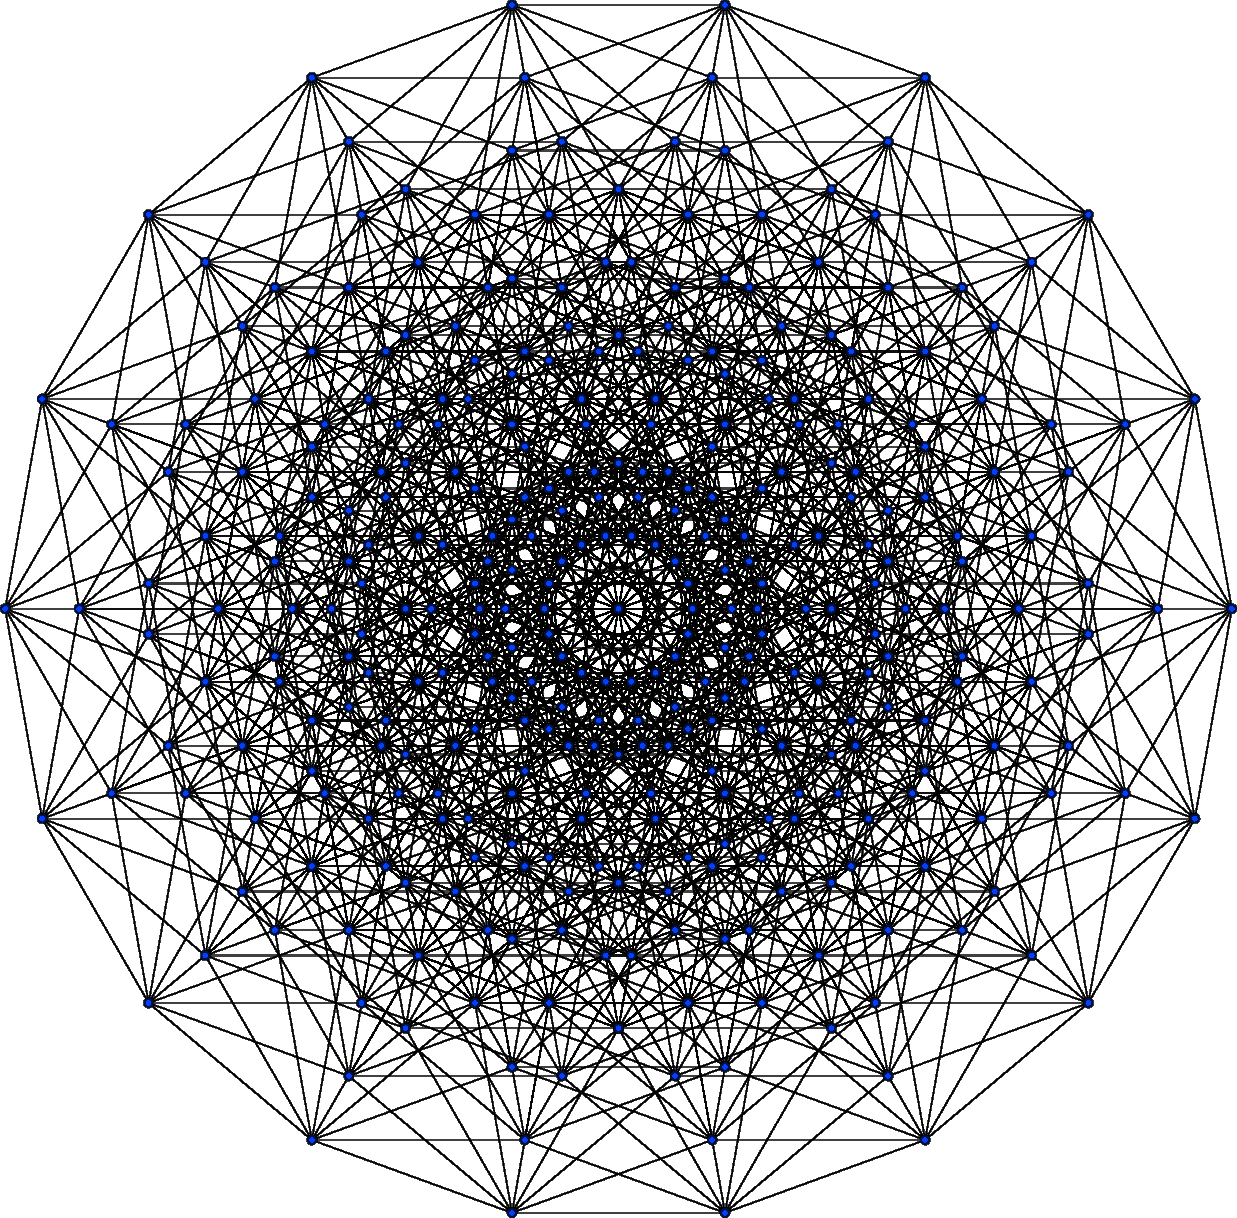
\includegraphics[scale=0.25]{images/q9.pdf}
\caption{Une projection de l'\textit{enneract} (9-hypercube)}
\end{figure}

\newpage

\subsection{Comparaison des différentes architectures}

À partir des résultats précédents, on peut manipuler les équations pour obtenir une estimation du diamètre, du degré des sommets, du nombre d'arêtes et de la bissection des différentes architectures étudiées jusqu'ici, directement en fonction du nombre de nœuds de calcul.

\begin{figure}[!h]
\begin{center}
\begin{tabular}{l|l|l|l|l}
Architecture & Diamètre & Degré & Nombre d'arêtes & Bissection \\ 
\toprule
Graphe complet & $1$ & $n-1$ & $\frac{n(n-1)}{2}$ & $\approx \frac{n^2}{4}$ \\ 
Grille de dimension $d$ & $d(n^{1/d}-1)$ & $2d$ & $dn(1-n^{-1/d})$ & $\approx n^{1-1/d}$ \\
Grille de dimension $2$ & $2(\sqrt{n}-1)$ & $4$ & $2(n-\sqrt{n})$ & $\approx \sqrt{n}$ \\ 
Grille d'arbres bidimensionnelle & • &  • & • & • \\ 
Hypercube & $\log_2 n$ & $\log_2 n$ & $n\log_2 n\frac{1}{2}$ & $\frac{n}{2}$ \\ 
\end{tabular}
\end{center}
\caption{Comparaison des architectures pour $n$ nœuds}
\end{figure}

On constate que l'hypercube offre les meilleurs diamètres et bissection, au détriment d'un degré non constant et d'arêtes plus nombreuses et plus longues par rapport à une grille classique, ce qui implique un câblage plus complexe et coûteux. Cela reste néanmoins une architecture de choix à l'heure actuelle.

\subsection{Implémentation du tri fusion}

\subsection{Quelques autres exemples d'algorithmes}